\documentclass[a4paper]{article}
\usepackage[dutch]{babel}
\usepackage[pdftex]{graphicx}
\usepackage{color}
\usepackage{url}
\usepackage{listings}
\usepackage{geometry}
\usepackage[toc]{glossaries}

\title{kplot --- Een stageproject over workflows}
\author{Koen Crolla \and Herman Bruyninckx (mentor)}
\date{15 juni 2012}

\makeglossaries
\newglossaryentry{REST}
{
    name=REST,
    description={\emph{REpresentational State Transfer}}
}

\newglossaryentry{SOAP}
{
    name=SOAP,
    description={Oorspronkelijk \emph{Simple Object Access Protocol},
                 tegenwoordig zonder betekenis}
}

\newglossaryentry{BPEL}
{
    name=BPEL,
    description={\emph{Business Process Execution Language}}
}

\newglossaryentry{WSDL}
{
    name=WSDL,
    description={\emph{Web Service Definition Language} (versie $\le$1.1),
                 \emph{Web Service Description Language} (versie $\ge$2.0)}
}

\newglossaryentry{RDF}
{
    name=RDF,
    description={\emph{Resource Description Framework}}
}

\newglossaryentry{SPARQL}
{
    name=SPARQL,
    description={\emph{\gls{SPARQL} Protocol and \gls{RDF} Query Language}}
}

\newglossaryentry{W3C}
{
    name=W3C,
    description={\emph{World Wide Web Consortium}}
}

\newglossaryentry{HTTP}
{
    name=HTTP,
    description={\emph{Hypertext Transfer Protocol}}
}

\newglossaryentry{HTTPS}
{
    name=HTTPS,
    description={\emph{\gls{HTTP} Secure}}
}

\newglossaryentry{API}
{
    name=API,
    description={\emph{Application/Programmer Interface}}
}

\newglossaryentry{SQL}
{
    name=SQL,
    description={\emph{Structured Query Language}}
}

\newglossaryentry{GNU}
{
    name=GNU,
    description={\emph{\gls{GNU}'s Not Unix}}
}

\newglossaryentry{URI}
{
    name=URI,
    description={\emph{Uniform Resource Identifier}}
}

\newglossaryentry{URL}
{
    name=URL,
    description={\emph{Uniform Resource Locator}}
}

\newglossaryentry{HTML}
{
    name=HTML,
    description={\emph{Hypertext Markup Language}, of misschien
                 \emph{Hypertext Meta Language}}
}

\newglossaryentry{YAWL}
{
    name=YAWL,
    description={\emph{Yet Another Workflow Language}}
}

\newglossaryentry{WSGI}
{
    name=WSGI,
    description={\emph{Web Server Gateway Interface}}
}

\newglossaryentry{XML}
{
    name=XML,
    description={\emph{eXtensible Markup Language}}
}


\begin{document}

\begin{titlepage}

\maketitle
\thispagestyle{empty}

\setcounter{tocdepth}{2}
\tableofcontents

\end{titlepage}

\section{Inleiding}

Dit stageproject, met de steeds minder toepasselijke naam {\tt kplot}, bekeek
mogelijkheden tot het verbeteren van wetenschappelijke workflows aan de KU
Leuven. Momenteel verlopen die vrij ad-hoc en misschien minder effectief dan
mogelijk, en we zouden hier graag enige standaardisering en stroomlijning in
brengen.

In de eerste instantie keken we naar ``{\it numerieke clients}''---hiermee
bedoelen we programma's of frameworks die vooral dienen om data te genereren
en te verwerken---en hoe we de {\bf opslag van data} (sectie \ref{sec:storage})
en het {\bf plotten van grafieken} (sectie \ref{sec:plotter}) konden
ontkoppelen, onder andere omdat andere programma's dit beter kunnen, maar ook
om een uniforme infrastructuur tussen clients te kunnen delen. We beoogden een
min of meer peer-to-peermodel (figuur~\ref{fig:model}) met een centrale
dataopslag en plotting clients die conceptueel vrij los staan van de numerieke
clients (sectie \ref{sec:numclient}).

\begin{figure}[ht]
  \label{fig:model}
  \centering
  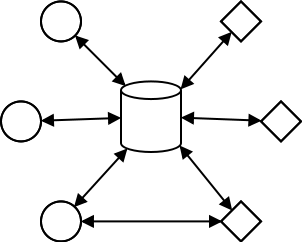
\includegraphics[width=2in]{model.png}
  \caption{Beoogd peer-to-peermodel}
\end{figure}

Daarna gingen we kijken naar nuttige manieren om onze datasets zoek- \'en
vindbaar te maken voor derden, en belandden zo bij het {\bf Linked Open Data}
concept van het \gls{W3C} (sectie \ref{sec:rdf}).

Tenslotte bekeken we hoe dit alles past binnen {\bf workflow engines}, en wat
er zoal bestaat op dat vlak (sectie \ref{sec:workflow}).

{\it Proof of concept} implementaties zijn voorzien waar mogelijk nuttig. Deze
code is niet geschikt voor gebruik in productie. Bij de beschrijving zijn
dependencies ge\"enumereerd bij naam van de relevante Debian Squeeze packages.

\newpage

\section{Storage}
\label{sec:storage}

De storage server, die het opslaan van de datasets gaat overnemen, staat vrij
centraal, dus daar zijn we mee begonnen. Voor de communicatie hebben we gekozen
voor \gls{HTTP}, omdat dit een goed ondersteund, algemeen bekend protocol is.
Mits redelijke keuze van libraries krijgen we ook veel nuttige dingen zoals
compressie (met {\tt Content-Encoding}), encryptie (\gls{HTTPS}), en zelfs
authenticatie (\gls{HTTPS}, basic/digest access authentication) gratis of bijna
gratis.

\subsection{Interfaces}

Nog een voordeel van \gls{HTTP} is dat er veel geteste idiomen bestaan voor web
services, zodat we het wiel niet helemaal opnieuw moeten gaan uitvinden. In de
eerste instantie hebben we gekozen voor \gls{REST} als model, omdat dit heel
natuurlijk leek voor het soort data dat we willen opslagen en de acties die we
erop willen uitvoeren. De \gls{REST} \gls{API} is beschreven in appendix
\ref{app:storage}.

Wanneer we later workflow engines gingen bekijken, bleek echter dat hoewel web
services een integraal deel uitmaken van \gls{BPEL} (zie sectie
\ref{sec:workflow}), in de praktijk vooral \gls{SOAP} web services werden
ondersteund. Daarom hebben we ook een \gls{SOAP} endpoint toegevoegd, en een
beschrijving hiervan in \gls{WSDL} 1.1.

Onze peers maken momenteel gebruik van de \gls{REST} interface, terwijl de
workflow engines gebruik maken van de \gls{SOAP} interface. Het lijkt ons niet
nuttig om \'e\'en van beide te schrappen ten voordele van de andere;
programmatisch is het veel handiger om met \gls{REST} te werken, maar onze
workflow engines kunnen nu eenmaal beter om met \gls{SOAP}.

\subsection{Concepten}

De structuur van de data in de storage zelf is vrij eenvoudig: een
{\bf dataset} heeft een ID en wat metadata (een titel, een label voor de X-as
en de Y-as, misschien een auteur en dergelijke), en \'e\'en of meerdere
hoeveelheden {\bf data} (die voor de storage server zelf opaak zijn).

Wanneer die data verandert door toedoen van een client wordt de nieuwe data
opgeslagen en gemarkeerd als zijnde de meest recente {\bf revisie}; de oude
data wordt niet gewist. Oudere data kan worden gemarkeerd als zijnde de meest
recente door bepaalde \gls{API}-methodes (appendix~\ref{app:storage}) die gaan
werken op timestamps of string labels ({\bf tags}) die de clients zelf gaan
toepassen.

\subsection{Implementatie}

\begin{tabular}{rl}
    {\bf Locatie:}      &   {\tt \$REPO/storage} \\
    {\bf Dependencies:} &   {\tt postgresql}, {\tt python},
                            {\tt python-psycopg2}
\end{tabular}

\vspace{.05in}

Als {\it proof of concept} hebben we gekozen voor een implementatie in Python,
als \gls{WSGI}-module, onder andere omdat dit even gemakkelijk als stand-alone
script kan worden uitgevoerd als gebruikt als normale module in een volwaardige
webserver, wat testen vergemakkelijkt. Voor de eigenlijke opslag van data
gebruiken we een Postgre\gls{SQL} databank, waarin twee tabellen zijn
aangemaakt volgens {\tt create.sql}.

Om de storage server te starten, maak de databank zelf eerst met de hand aan,
pas eventueel {\tt config.py} aan en run dan {\tt db.py} (liefst met een lege
environment: {\tt env - ./db.py}).

Let wel: het \gls{SOAP} endpoint is niet gereflecteerd in deze implementatie,
omdat de code van te lage kwaliteit was om nuttig te zijn. Dit ligt
gedeeltelijk aan het feit dat Python libraries voor \gls{SOAP} eerder gericht
zijn op pure \gls{SOAP} web services, en niet (gemakkelijk) als nagedachte
kunnen worden toegevoegd aan een bestaande \gls{REST} service. Om goed te zijn
zou de hele storage service misschien beter geherimplementeerd worden
beginnende als \gls{SOAP} service, waar dan een \gls{REST} service wordt aan
toegevoegd.

\subsection{Open vragen}
\label{subsec:storagetodo}

Er zou moeten gekeken worden naar nuttige werkwoorden op ons soort datasets, die
dan in \gls{SOAP} kunnen worden ge\"implementeerd. In eerste instantie zou het
goed zijn om alle operaties van de \gls{REST} interface te dupliceren in
\gls{SOAP}.

Ook kan Postgre\gls{SQL} eventueel vervangen worden door andere oplossingen. We
hebben eigenlijk geen volledige relationele databank nodig, en niet-relationele
opties als MongoDB kunnen misschien sneller zijn. Tests zullen moeten uitmaken
of Postgre\gls{SQL} daadwerkelijk te traag is.

Verder zou het misschien nuttig zijn om te kijken naar mogelijkheden tot
authenticatie van clients. Momenteel kan iedereen alle datasets manipuleren;
in de praktijk is dit misschien niet zo'n goed idee.

Tenslotte zou er ook nog een manier moeten zijn om peers bij te houden. Als we
strict het peer-to-peermodel volgen zouden peers als numerieke clients (zie
sectie~\ref{subsec:python}) zich moeten kunnen registreren voor bepaalde
updates, en zou de storage server zelf updates moeten gaan pushen naar deze
subscribers (en subscribers verwijderen uit de lijst wanneer ze niet meer
bereikbaar zijn). Of dit inderdaad heel nuttig is is ook de vraag.

\newpage

\section{Numerieke clients}
\label{sec:numclient}

Met {\it numerieke clients} bedoelen we programma's als MATLAB of frameworks
als SciPy die bedoeld zijn om data te genereren en te verwerken. Vaak hebben
deze clients de mogelijkheid om zelf data te gaan plotten op grafiek of op te
slaan in een databank, maar dit willen we dus ontkoppelen. We schrijven dus
zelf een library of plugin om met onze storage server (sectie
\ref{sec:storage}) en plotting clients (sectie~\ref{sec:plotter}) te gaan
werken.

\subsection{\gls{GNU} Octave}

Eerst hebben we gekozen voor \gls{GNU} Octave, omdat Octave, MATLAB en Scilab
allemaal populair en relatief intercompatibel zijn; een model dat werkt in
\gls{GNU} Octave zou dus ook moeten kunnen werken in MATLAB en Scilab.

Onze library spiegelde zich aan bestaande functionaliteit: het ingebouwde
{\tt plot} werd {\tt kplot},\footnote{Vandaar.} {\tt title} werd {\tt ktitle},
{\tt xlabel} en {\tt ylabel} werden {\tt kxlabel} en {\tt kylabel}, enzovoort.
Dit werkte om de plottingfunctionaliteit te ontkoppelen, maar bleek niet meteen
bruikbaar voor de storagefunctionaliteit: expliciete stores en loads waren wel
mogelijk, maar als andere clients de data in de storage zouden veranderen, zou
er geen transparante manier zijn om dit transparent voor de gebruiker te
reflecteren aan de numerieke clients.

\subsubsection{Implementatie}

\begin{tabular}{rl}
    {\bf Locatie:}      & {\tt \$REPO/numeriek/octave} \\
    {\bf Dependencies:} & {\tt build-essential}, {\tt octave}, {\tt python}
\end{tabular}

\vspace{.05in}

Om het eenvoudig te houden wordt het meeste werk niet gedaan door de C++
library, maar door een extern Pythonscript dat aangeroepen wordt vanuit de
library.

Plaats {\tt kplotter.py} ergens in het {\tt PATH}, en roep {\tt make} aan
zonder argumenten om de package {\tt kplot.tar.gz} te bouwen. Start dan
\gls{GNU} Octave in dezelfde directory en installeer de package met
``{\tt pkg install kplot.tar.gz}''.

De package implementeert de functies {\tt kplot}, {\tt ktitle}, {\tt kxlabel},
{\tt kylabel}, {\tt kpurge\_tmp\_files} en {\tt kplot\_server}. De eerste vijf
bootsen de ingebouwde functies zonder {\tt k} na; de laatste toont of verandert
de ingestelde plotting server, naargelang hij zonder of met argument wordt
aangeroepen.

Let op: {\tt kplotter.py} gaat uit van een oudere versie van de storage server
(zie sectie \ref{sec:dygraphs}) en zal dus niet werken. De code is enkel ter
illustratie. 

\subsection{Python}
\label{subsec:python}

Vervolgens zijn we overgestapt naar Python. Datasets voorstellen als objecten
bleek heel natuurlijk, en door de ``magische'' methoden
{\tt \_\_getattribute\_\_}, {\tt \_\_setattr\_\_} en {\tt \_\_delattr\_\_}
\footnote{\url{http://docs.python.org/reference/datamodel.html#customizing-attribute-access}}
te overschrijven konden we informatie heel transparent gesynchroniseerd houden
met de storage server. Dit loste alle problemen op: metadata manipuleren werd
gewoon een kwestie van instantievariabelen aanpassen, data gaan plotten was
gewoon maar een method call op het datasetobject, en we konden met meerdere
onafhankelijke datasets tegelijk gaan werken.

Het was wel nog steeds eerder een client/servermodel dan een peer-to-peermodel:
telkens wanneer de gebruiker aan een instantievariabele kwam werd een
\gls{HTTP}-verzoek gestuurd naar de storage server om te kijken of die
veranderd was, en indien ja, om de nieuwe informatie af te halen. Dit kon
worden opgelost met een lokale daemon, die gespawnd wordt wanneer de library
wordt geladen. Deze daemon gaat zich registreren bij de storage server (maar
zie sectie \ref{subsec:storagetodo}), en de eigenlijke library gaat nog wel op
dezelfde manier pullen, maar enkel lokaal van de daemon, niet meer van de
storage server over het netwerk.

\subsubsection{Implementatie}

\begin{tabular}{rl}
    {\bf Locatie:}      & {\tt \$REPO/numeriek/python} \\
    {\bf Dependencies:} & {\tt python}
\end{tabular}

\vspace{.05in}

Het is de bedoeling dat {\tt kplot.py} wordt geimporteerd als module in een
Pythonsessie (interactief of als script). Volledige documentatie is dan
toegankelijk door middel van {\tt help(kplot)}. Uiteindelijk is het de
bedoeling dat de {\tt Dataset}-klasse omkan met datatypes van de SciPy en
NumPy libraries, maar momenteel is dit niet het geval.

Let wel: het hele gebeuren met de daemon is dus niet ge\"implementeerd; alle
communicatie gebeurt rechtstreeks met de storage server, volgens het
client/servermodel.

\subsection{Open vragen}

De mogelijkheid om vanuit de numerieke client beperkt het gedrag van een
plotting client te be\"invloeden (verder dan alleen maar het opstarten ervan)
zou wel nuttig zijn, en in lijn met ons peer-to-peermodel.

\newpage

\section{Plotting clients}
\label{sec:plotter}

Plotting clients zijn ook maar gewoon peers in ons model. Zij gaan het plotten
van data op grafiek verzorgen. We zouden graag niet enkel statische plots
hebben, maar de mogelijkheid om filters en fits en dergelijke toe te passen op
de data, en die veranderingen gereflecteerd te zien in de storage server.

\subsection{dygraphs}
\label{sec:dygraphs}

In de eerste instantie gebruikten we de Javascript library dygraphs, en ging
de storage server zelf een webpagina tonen met de grafiek op (dit kon even
goed door een aparte webserver gedaan worden, maar de extra overhead van een
kleine statische pagina was verwaarloosbaar).

Het nadeel was dat dygraphs enkel voor weergave zorgt, en natuurlijk niet
toelaat om de data op de grafiek aan te passen.

\subsection{Kst}

Daarom zijn we dus overgestapt naar het veel krachtigere Kst 2, dat ingebouwde
ondersteuning heeft voor allerlei manieren om data op grafiek te manipuleren
en ook al gebruikt werd aan het departement.

Ondersteuning toevoegen is in principe maar een kwestie van een
{\it datasource} plugin te schrijven. Kst kan zelf al gaan pollen of data niet
veranderd is, dus dat deel krijgen we gratis. Het enige probleem is toegang
krijgen tot door Kst gewijzigde data wanneer filters of fits worden toegepast,
en deze nieuwe data communiceren naar de storage server toe.

Dit bleek een probleem. Kst zelf slaat die informatie op een hoog niveau op
als een lijst verandering aan de data, en niet als veranderde data zelf (wat
ook hetgene is dat Kst toelaat om met zulke grote datasets te werken), en als
de mogelijkheid bestaat om wel aan die data te kunnen, dan is die niet
gereflecteerd in de heel gebrekkige documentatie.

Helaas hebben we hier dan ook geen implementatie voor; de code was van te lage
kwaliteit om zelfs als {\it proof of concept} te dienen. Ondernemende lezers
raden we aan te beginnen met te kijken naar bestaande datasource plugins in de
Kst source tree en zelf iets te proberen. Misschien is het toch lonender om met
Kst 1 te werken; dat heeft zijn eigen problemen, maar ook documentatie.

\newpage

\section{Linked Open Data}
\label{sec:rdf}

We zouden onze datasets natuurlijk ook graag terug kunnen vinden achteraf, en
misschien zelfs vindbaar maken voor derde partijen. In dit kader hebben we het
{\it Linked Open Data} concept van het \gls{W3C} bekeken.

{\it Linked data} betekent dat resources die we willen blootstellen
ge\"identificeerd worden door een \gls{URI}, en dat we wanneer we die \gls{URI}
volgen ({\it dereferencing}) daadwerkelijk relevante informatie terugvinden.
{\it Open data} betekent dat alle informatie beschikbaar is in open formaten
en onder een open licentie.

In de praktijk komt Linked Open Data erop neer dat we metadata over onze
datasets gaan opslaan als \gls{RDF}-expressies in een zogehete
{\it triplestore}. Een \gls{RDF}-expressie bestaat uit drie
componenten---een onderwerp, een predicaat, en een lijdend voorwerp
({\it subject-predicate-object}):\footnote{
    Vandaar de naam {\it triplestore}. Er bestaat ook een extensie met een
    vierde component (context) die dan in een {\it quadstore} wordt opgeslagen,
    maar dit biedt voor ons geen toegevoegde waarde.
}

\begin{quotation}
    {\it lucht heeft-kleur blauw .}\footnote{
        Deze syntax is de {\it N-Triples} serialisatie voor \gls{RDF} (en isi
        ook geldig {\it Turtle} en {\it Notation3}). Er bestaat onvermijdelijk
        ook een \gls{XML}-serialisatie: \gls{RDF}/\gls{XML}.
    }
\end{quotation}

Of concreter:

\begin{quotation}
    {\it \url{<http://www.example.com/dataset/1234>}

         \url{<http://www.example.com/ontology#x-label>}

         ``tijd'' .}
\end{quotation}

Onze triplestore heeft ook een {\it \gls{SPARQL} endpoint}; dit is een plaats
waar \gls{SPARQL}-queries kunnen worden uitgevoerd op de data in de server.
\gls{SPARQL} is een op \gls{SQL} gebaseerde taal om \gls{RDF}-databanken te
ondervragen.

Omdat het gebruikspatroon van deze triplestore sterk verschilt van onze storage
server, hebben we ervoor gekozen om hem als een aparte server te implementeren.
De volledige \gls{API} ervan is beschreven in appendix~\ref{app:rdf}. Er zijn
methodes voorzien om data van de storage server te ``publiceren'' naar de
\gls{RDF} server, en om datasets in te laden van de \gls{RDF} server naar de
storage server. Voor details, zie appendix~\ref{app:storage} en de {\tt help()}
voor de Python module.

\subsection{Implementatie}

\begin{tabular}{rl}
    {\bf Locatie:}      & {\tt \$REPO/rdf}      \\
    {\bf Dependencies:} & {\tt postgresql}, {\tt python}, {\tt python-mako},
                          {\tt python-psycopg2}, {\tt rdflib}
\end{tabular}

\vspace{.05in}

Er bestaan al softwarepaketten voor \gls{RDF} servers (OpenLink Virtuoso is er
\'e\'en die we in detail bekeken hebben; de niet-libre versie hiervan wordt
bijvoorbeeld gebruikt door DBpedia), maar ze doen meestal nog veel meer en
configuratie bleek niet triviaal. Uiteindelijk was het eenvoudiger om het zelf
te doen, met \'e\'en van de libraries die hiervoor voorhanden zijn.

Onze implementatie is weer een \gls{WSGI}-module in Python, en gebruikt
Postgre\gls{SQL} als {\it backing store}. Eerst gebruikten we Python bindings
voor de Redland \gls{RDF} Libraries, maar uiteindelijk zijn we overgestapt op
het pure-Python {\tt rdflib} omdat de \gls{API} hiervan Pythonischer was en de
documentatie iets beter. We gebruiken ook Mako templates voor de \gls{HTML}.

Om de \gls{RDF} server op te starten, pas {\tt config.py} aan en run dan
{\tt rdf.py} (liefst met een lege environment: {\tt env - ./rdf.py}).
{\tt rdflib} zal zelf de nodige tabellen aanmaken.

\subsection{Open vragen}

Er zou nader moeten bekeken welke metadata nuttig zou kunnen zijn. Momenteel
houden we enkel een {\tt rdfs:label} (titel van de dataset), {\tt x-label},
{\tt y-label} en data zelf bij. Dingen als auteur(s) en datum(s) zijn verder
vrij vanzelfsprekend; wat nog?

Een gebruiksvriendelijkere manier om op datasets te zoeken dan enkel maar rauwe
\gls{SPARQL} zou waarschijnlijk ook handig zijn.

\newpage

\section{Workflow engines}
\label{sec:workflow}

Omdat het project om het verbeteren van wetenschappelijke workflows draaide,
zijn we tenslotte ook gaan kijken naar workflow engines. Dit zijn programma's
die gebruikers toelaten om zelf workflows samen te stellen uit bepaalde
bouwstenen, en die workflows uit te voeren.

Een ``traditionele'' workflow engine implementeert \gls{BPEL}. Conceptueel is
\gls{BPEL} een standaard die workflows gaat zien als een reeks bouwstenen met
inputs en outputs die aan elkaar gekoppeld kunnen worden, met een paar extra
mogelijkheden zoals loops, retries, etc. De bouwstenen zijn vaak
\gls{SOAP}-acties die beschreven zijn in \gls{WSDL} (een workflow engine zal
een \gls{WSDL}-beschrijving van een web service importeren om zo de beschreven
acties als primitieven te kunnen gebruiken), maar kunnen vaak ook lokale
programma's of speciale ingebouwde services zijn (bijvoorbeeld een R shell,
JavaBeans, of zelfs andere workflows).\footnote{De \gls{BPEL}-standaarden zijn
ambitieus en specifiek, en een uitgebreide behandeling ervan ligt buiten de
scope van dit verslag. Voor meer informatie, zie het Internet.}

\begin{figure}[ht]
  \centering
  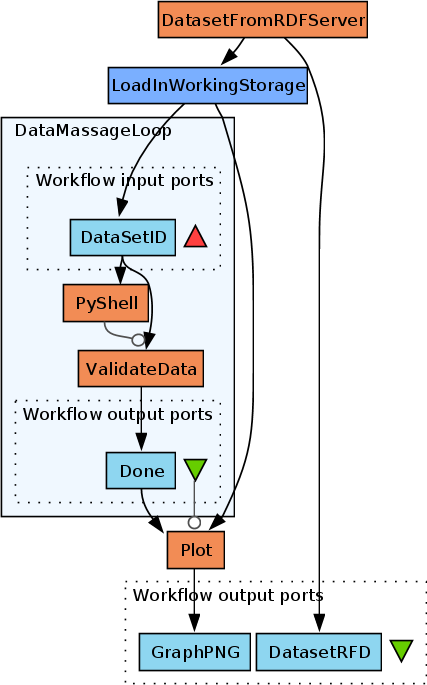
\includegraphics[width=2in]{workflow.png}
  \caption{Voorbeeld van een workflow in Taverna}
\end{figure}

We hebben vier workflow engines bekeken: Orchestra, \gls{YAWL}, Kepler en
Taverna. Uiteindelijk hebben we gekozen voor Taverna als zijnde de nuttigste.
Hier volgt een korte bespreking van de relevante punten.

\subsection{Orchestra}

Orchestra is een vrij traditionele workflow engine gebaseerd op \gls{BPEL}. De
belangrijkste onderscheidende eigenschap is het feit dat het draait op een web
server en de gebruikersinterface een webpagina is. Uiteindelijk is dit de reden
geworden dat we Orchestra verworpen hebben: het maakt het runnen van lokale
scripts onmogelijk, tenzij de gebruiker Orchestra zelf ook lokaal gaat draaien.
Aangezien dat Orchestra een vrij zware Java-applicatie is die niet triviaal te
deployen valt, leek dit onrealistisch.

\subsection{\gls{YAWL}}

\gls{YAWL} stapt af van \gls{BPEL}, maar is duidelijk meer gericht naar
bedrijfsprocessen. Conceptueel is het goed onderbouwd met gepubliceerd
onderzoek, maar in de praktijk blijken de verschillen met \gls{BPEL} weinig
relevant voor onze doeleinden en vaak onnodig verwarrend.

Het feit dat \gls{BPEL} een levendig ecosysteem heeft met veel bestaande
projecten en web services, terwijl \gls{YAWL} enkel \gls{YAWL} zelf heeft, is
nog een reden waarom we deze workflow engine uiteindelijk verworpen hebben.

\subsection{Kepler}

Kepler stapt ook van \gls{BPEL} af, en is specifiek ontworpen voor
wetenschappelijke workflows. Het onderscheidt zich door het gebruik van
{\it Actors}, die web services gaan vervangen als fundamentele bouwstenen van
de workflow, en {\it Directors}, die be\"invloeden hoe workflows zich
fundamenteel gaan gedragen.

Uiteindelijk geeft dit weinig toegevoegde waarde, en de grote hoeveelheid
Directors, elk met vrij vage of zelfs volledig ontbrekende beschrijvingen van
hun functie, verwart alleen maar.

\subsection{Taverna}

Taverna is een ``traditionele'' \gls{BPEL} workflow engine die, in
tegenstelling tot Orchestra, een gewone lokale applicatie is. Er is weinig
interessant aan, en dat is uiteindelijk zijn sterkste punt: alles werkt heel
intuitief en plaats niet te veel cognitieve stressors op de gebruiker. Daarom
is het uiteindelijk onze keuze geworden.

Taverna ondersteunt trouwens ook wel REST services, zij het niet op de
automatische manier met het importeren van WSDL; gebruikers moeten altijd zelf,
manueel \gls{URL}s en inputs/outputs defini\"eren. Voor eenvoudige acties is
dit toch nuttig.

\subsection{Open vragen}

Vragen zijn er zo niet, maar er is nog werk te doen. Het nut van workflow
engines hangt sterk samen met de kwaliteit van het \gls{SOAP} endpoint van de
storage server (sectie~\ref{subsec:storagetodo}), en effectief gebruik van
workflows zal ook minstens gedeeltelijk afhangen van de kwaliteit van de
gebruikspatronen; het zou dus nuttig zijn om hier een paar van te identificeren
en te documenteren.

Een voorbeeld is het cre\"eren van een Python shell om de library van sectie
\ref{subsec:python} te gebruiken; dit kan in Taverna door met behulp van de
Tool service template een terminalvenster te openen dat automatisch een Python
shell start met een dataset ID in de environment of als argument:

\begin{quote}
    {\tt gnome-terminal -x python - \%\%DATASET\%\%}
\end{quote}

Als de gebruiker in de shell dan gewoon een nieuw {\tt Dataset}-object aanmaakt
zonder argumenten, zal de library zelf gaan kijken naar de environment of de
command line argumenten en de relevante dataset inladen.

Dit is een nuttig patroon dat gedocumenteerd moet worden voor de gebruiker, en
zo zijn er denkbaar nog.

\newpage

\section{Conclusie}

Het zou duidelijk moeten zijn dat er nog ruimte is om verder te gaan. De
plotting clients, waarmee het hele project eigenlijk begon, zijn nog
onbestaande, en de rest is zeker voor verbetering vatbaar.

Ik hoop dat er toch waardevolle vooruitgang is geboekt, en wens degene die
hiermee verder gaat veel geluk.

\newpage

\appendix
\section{Working Storage \gls{API}}
\label{app:storage}

\begin{itemize}
  \item {\tt\large\bf /}
    \begin{description}
      \item[POST, PUT] \hfill \\
        {\bf Parameters}
        \begin{itemize}
          \item {\tt title} {\it (optioneel)}: titel van de dataset
          \item {\tt x-label} {\it (optioneel)}: label voor de X-as
          \item {\tt y-label} {\it (optioneel)}: label voor de Y-as
          \item {\tt data}: data (formaat ``$x_1,y_1;x_2,y_2;\ldots$'')
        \end{itemize}
        Maakt een nieuwe dataset aan met de opgegeven metadata. Geeft
        ``{\it dataset\_id},\linebreak[4]{\it timestamp}'' terug.
    \end{description}
  \item {\tt\large\bf /load}
    \begin{description}
      \item[POST, PUT] \hfill \\
        {\bf Parameters}
        \begin{itemize}
          \item {\tt uri}: \gls{URI} van een dataset in een \gls{RDF}-server
                (sectie~\ref{sec:rdf})
        \end{itemize}
        Maakt een nieuwe dataset aan op basis van de gegevens aan de \gls{URI}.
    \end{description}
  \item {\tt\large\bf /{\it dataset\_id}}
    \begin{description}
      \item[GET] \hfill \\
        Toont de meest recente informatie geassocieerd met dataset
        {\it dataset\_id} in JSON-formaat.
      \item[POST] \hfill \\
        {\bf Parameters}
        \begin{itemize}
          \item {\tt title} {\it (optioneel)}: titel van de dataset
          \item {\tt x-label} {\it (optioneel)}: label voor de X-as
          \item {\tt y-label} {\it (optioneel)}: label voor de Y-as
          \item {\tt data} {\it (optioneel)}: data (formaat
                ``$x_1,y_1;x_2,y_2;\ldots$'')
        \end{itemize}
        Wijzigt de opgegeven metadata geassocieerd met dataset {\it dataset\_id}
        en geeft de timestamp van de huidige revisie terug.
      \item[PUT] \hfill \\
        Hetzelfde als POST, maar geeft ``400 Bad Request'' terug als het
        metadatum al bestaat voor de dataset.
      \item[DELETE] \hfill \\
        Wist dataset {\it dataset\_id}.
    \end{description}
  \item {\tt\large\bf /{\it dataset\_id}/timestamp}
    \begin{description}
      \item[DELETE] \hfill \\
        Wist enkel revisie {\it timestamp} van dataset {\it dataset\_id}.
    \end{description}
  \item {\tt\large\bf /{\it dataset\_id}/diff}
    \begin{description}
      \item[GET] \hfill \\
        Geeft de timestamp van de meest recent revisie van dataset
        {\it dataset\_id} terug.
    \end{description}
  \item {\tt\large\bf /{\it dataset\_id}/diff/{\it timestamp}}
    \begin{description}
      \item[GET] \hfill \\
        Geeft ``yes'' of ``no'' terug, naargelang de huidige revisie van
        dataset {\it dataset\_id} verschilt van {\it timestamp}.
    \end{description}
  \item {\tt\large\bf /{\it dataset\_id}/json}
    \begin{description}
      \item[GET] \hfill \\
        Toont de meest recente informatie geassocieerd met dataset
        {\it dataset\_id} in JSON-formaat.
    \end{description}
  \item {\tt\large\bf /{\it dataset\_id}/json/{\it timestamp}}
    \begin{description}
      \item[GET] \hfill \\
        Toont alle informatie geassocieerd met dataset {\it dataset\_id},
        revisie {\it timestamp}, in JSON-formaat.
    \end{description}
  \item {\tt\large\bf /{\it dataset\_id}/kst}
    \begin{description}
      \item[GET] \hfill \\
        Toont de meest recente informatie geassocieerd met dataset
        {\it dataset\_id} in een formaat waar de Kstplugin mee overweg kan.
    \end{description}
  \item {\tt\large\bf /{\it dataset\_id}/kst/{\it timestamp}}
    \begin{description}
      \item[GET] \hfill \\
        Toont de informatie geassocieerd met dataset {\it dataset\_id},
        revisie {\it timestamp}, in een formaat waar de Kstplugin mee overweg
        kan.
    \end{description}
  \item {\tt\large\bf /{\it dataset\_id}/title}
    \begin{description}
      \item[DELETE] \hfill \\
        Wist de titel geassocieerd met dataset {\it dataset\_id}.
    \end{description}
  \item {\tt\large\bf /{\it dataset\_id}/x-label}
    \begin{description}
      \item[DELETE] \hfill \\
        Wist de title van de X-as geassocieerd met dataset {\it dataset\_id}.
    \end{description}
  \item {\tt\large\bf /{\it dataset\_id}/y-label}
    \begin{description}
      \item[DELETE] \hfill \\
        Wist de titel van de Y-as geassocieerd met dataset {\it dataset\_id}.
    \end{description}
  \item {\tt\large\bf /{\it dataset\_id}/tags}
    \begin{description}
      \item[GET] \hfill \\
        Toont alle tags geassocieerd met dataset {\it dataset\_id}, gescheiden
        door newlines ({\tt \char`\\n}), oudste eerst.
    \end{description}
  \item {\tt\large\bf /{\it dataset\_id}/tag}
    \begin{description}
      \item[POST] \hfill \\
        {\bf Parameters:}
        \begin{itemize}
          \item {\tt tag}
        \end{itemize}
        Associeert {\tt tag} met de meest recente revisie van dataset
        {\it dataset\_id}.
    \end{description}
  \item {\tt\large\bf /{\it dataset\_id}/rewind}
    \begin{description}
      \item[POST] \hfill \\
        {\bf Parameters:}
        \begin{itemize}
          \item {\tt timestamp} \\
          OF
          \item {\tt tag}
        \end{itemize}
        Markeert de revisie ge\"identificeerd door {\tt timestamp} of {\tt tag}
        van dataset {\it dataset\_id} als zijnde de meest recente.
    \end{description}
\end{itemize}

\section{\gls{RDF} Server \gls{API}}
\label{app:rdf}

\begin{itemize}
  \item {\tt\large\bf /}
    \begin{description}
      \item[GET] \hfill \\
        Toont de voorpagina, met wat informatie over de \gls{RDF} server en een
        link naar de \gls{SPARQL} endpoint.
    \end{description}
  \item {\tt\large\bf /dataset/{\it dataset\_id}}
    \begin{description}
      \item[GET] \hfill \\
        Geeft alle metadata geassocieerd met dataset {\it dataset\_id} terug
        als \gls{RDF}/\gls{XML}.
      \item[DELETE] \hfill \\
        Verwijdert de dataset volledig.
    \end{description}
  \item {\tt\large\bf /ontology}
    \begin{description}
      \item[GET] \hfill \\
        Toont de ontologie van de \gls{RDF} server als \gls{RDF}/\gls{XML}.
    \end{description}
  \item {\tt\large\bf /sparql}
    \begin{description}
      \item[GET] \hfill \\
        Toont \gls{HTML}-formulier voor het \gls{SPARQL} endpoint.
      \item[POST] \hfill \\
        {\bf Parameters:}
        \begin{itemize}
          \item {\tt query}: \gls{SPARQL} query
          \item {\tt type} {\it (optioneel)}: gewenste formaat ({\tt html},
                {\tt xml}, {\tt triples})
        \end{itemize}
        Voert de query uit en geeft de resultaten terug in het gewenste formaat,
        of in \gls{RDF}/\gls{XML} wanneer er geen formaat gespecifieerd is.
    \end{description}
  \item {\tt\large\bf /submit}
    \begin{description}
      \item[POST, PUT] \hfill \\
        {\bf Parameters:}
        \begin{itemize}
          \item {\tt title}: titel van de dataset
          \item {\tt x-label} {\it (optioneel)}: label voor de X-as
          \item {\tt y-label} {\it (optioneel)}: label voor de Y-as
          \item {\tt data}: data (formaat ``$x_1,y_1;x_2,y_2;\ldots$'')
        \end{itemize}
        Cre\"eert een nieuwe dataset met opgegeven metadata. Geeft de \gls{URI}
        van de gecre\"eerde dataset terug.
    \end{description}
\end{itemize}


\section{Links}

\subsection*{Numerieke clients}

\begin{description}
    \item[\gls{GNU} Octave] \url{http://www.gnu.org/software/octave/}
    \item[MATLAB]           \url{http://www.mathworks.com/products/matlab/}
    \item[NumPy]            \url{http://numpy.scipy.org/}
    \item[Scilab]           \url{http://www.scilab.org/}
    \item[SciPy]            \url{http://www.scipy.org/}
\end{description}

\subsection*{Plotting clients}

\begin{description}
    \item[dygraphs]     \url{http://dygraphs.com/}
    \item[Kst]          \url{http://kst-plot.kde.org/}
    \item[matplotlib]   \url{http://matplotlib.sourceforge.net/}
\end{description}

\subsection*{Linked Open Data}

\begin{description}
    \item[OpenLink Virtuoso]            \url{http://virtuoso.openlinksw.com/}
    \item[rdflib]                       \url{http://www.rdflib.net/}
    \item[Redland \gls{RDF} Libraries]  \url{http://librdf.org/}
\end{description}

\subsection*{Workflow engines}

\begin{description}
    \item[Kepler]       \url{https://kepler-project.org/}
    \item[Orchestra]    \url{http://orchestra.ow2.org/}
    \item[Taverna]      \url{http://www.taverna.org.uk/}
    \item[WF4Ever]      \url{http://www.wf4ever-project.org/}
    \item[\gls{YAWL}]   \url{http://www.yawlfoundation.org/}
\end{description}

\printglossaries

\end{document}
